\documentclass[11pt,a4paper,final]{article}

\usepackage[T1]{fontenc}
\usepackage[utf8]{inputenc}
\usepackage[italian]{babel}
\usepackage{layaureo}
\usepackage{microtype}
\usepackage{fancyhdr}

\usepackage{tikz}
\usetikzlibrary{trees}

\usepackage{amsmath}
\usepackage{amsfonts}
\usepackage{amssymb}
\usepackage{graphicx}
%\usepackage{eurosym}
%\usepackage[usenames,dvipsnames]{color}
%\usepackage[left=2cm,right=2cm,top=2.5cm,bottom=3cm]{geometry}
%\usepackage{indentfirst}
\usepackage{hyperref}
%\usepackage{subcaption}
\usepackage{booktabs}
%\usepackage{multirow}
\usepackage{listings}
\usepackage{xspace}
\usepackage{caption}
\usepackage{subfig}



\definecolor{redUni}{RGB}{181,18,27}

\author{Marco Pezzutti - 1084411}
\title{Resequencing}
\date{}

\def\campo#1{\uppercase{\textit{#1}}\xspace}
\def\acronimo#1{\uppercase{#1}\xspace}
\def\script#1{\texttt{#1}\xspace}
\def\modo#1{\uppercase{#1}\xspace}
\def\comando#1{\uppercase{\texttt{#1}}\xspace}

\pagestyle{fancy}
\renewcommand{\headrulewidth}{0pt}
\fancyhead[RE, LO]{}
\fancyfoot{}
\fancyfoot[RO, LE]{\thepage{}}
\fancyfoot[RE, LO]{Resequencing - Progetto di Bioinformatica}
\renewcommand{\footrulewidth}{0.4pt}

\begin{document}
\begin{titlepage}
\begin{center}
\includegraphics[width=40mm]{immagini/Logo_Padova.png}\\[1cm]
\textcolor{redUni}{\textsc{\LARGE Università degli Studi di Padova}}\\[0.5cm]
\textcolor{redUni}{\textsc{\Large Dipartimento di Matematica}}\\[0.5cm]
\textcolor{redUni}{\textsc{\Large Corso di Laurea Magistrale in Informatica}}\\[2cm]
\textsc{\Large Progetto di Bioinformatica}\\[0.5cm]
\textsc{\large Anno 2014-2015} \\[1cm]
\rule{\linewidth}{0.3mm}\\[0.5cm]
{\huge \bfseries Resequencing}\\[0.3cm]
\rule{\linewidth}{0.3mm}\\[1cm]
\begin{minipage}{0.4\textwidth}
	\begin{flushleft}
	\emph{Autore:}\\
	\textsc{\large Pezzutti Marco}\\
	\end{flushleft}
\end{minipage}
\begin{minipage}{0.4\textwidth}
	\begin{flushright}
	\emph{Matricola:}\\
	\textsc{\large 1084411}\\
	\end{flushright}
\end{minipage}
\end{center}
\end{titlepage}

\tableofcontents
\listoffigures
\listoftables
\newpage

\section{Introduzione}
Ho scelto di svolgere il progetto sul \emph{resequencing} in quanto richiede lo studio e la comprensione degli aspetti basilari della materia: è necessario infatti aver compreso chiaramente i concetti biologici spiegati a lezione che riguardano funzione e struttura del \acronimo{dna} nonché il suo funzionamento.

Inoltre ritengo che questo sia un buon punto di partenza per affrontare una materia completamente nuova per me e che mi interessa molto sia dal punto di vista didattico che professionale.

Per poter svolgere nel modo corretto il progetto è stato molto importante capire a fondo la struttura dei file \acronimo{bam/sam}, utilizzando i manuali dedicati e passando molto tempo a leggere tali file cercando di capire gli aspetti peculiari e rilevanti per ottenere le informazioni desiderate.
\clearpage
\section{Strumenti utilizzati}
Lo svolgimento del progetto richiede di effettuare un analisi dei file \acronimo{bam} forniti con lo scopo di estrarre alcune informazioni presenti in essi; inoltre è stata lasciata libera scelta sugli strumenti da utilizzare e sulle informazioni da ricercare.

Di seguito verranno descritti gli strumenti che ho scelto di utilizzare e la motivazione che mi ha portato a questa decisione.

\begin{description}
\item[\textsc{Samtools}]: i \emph{samtools} sono un insieme di strumenti utili per la manipolazione di file in formato \acronimo{BAM/SAM} che consentono la visualizzazione, la conversione, l'unione, l'ordinamento e l'indicizzazione di un file; tali operazioni sono necessarie per ottenere un file di partenza che sia coerente con l'analisi che si vuole effettuare;
\item[\textsc{Python}]: la natura del progetto non richiede lo sviluppo di un software particolarmente complicato e interattivo, è sufficiente che sia in grado di leggere i file, effettuare alcuni calcoli e scrivere i risultati su nuovi file.

Per questo motivo la scelta è caduta su \emph{python}: è un linguaggio che consente di sviluppare velocemente script ed è dotato di una grande varietà di librerie, tipi e strutture dati che lo rendono molto flessibile e adatto a numerosi scopi;
\item[\textsc{Pysam}]: è una libreria wrapper di \emph{HTSlib\footnote{\url{http://www.htslib.org/}}} scritta per essere utilizzata con \emph{python} e che consente di leggere e scrivere le informazioni presenti nei \acronimo{bam/sam} file in modo rapido ed efficiente.
\item[\textsc{Gnuplot}]: è un software che consente di realizzare grafici a partire da funzioni o dati grezzi; nel progetto è stato usato per disegnare la lunghezza degli inserti trovati in modo da poter analizzare tali dati;
\item[\textsc{IGV}]: l'\emph{Integrative Genomic Viewer} è un programma che consente di visualizzare tracce contenenti dati genomici attraverso l'uso di diversi tipi di file tra i quali quelli in formato \emph{wiggle};
\item[\textsc{IGVtools}]: insieme di strumenti utili per la preparazione dei dati da visualizzare nel viewer;
\item[\textsc{Bash}]: per automatizzare il processo di ottenimento dei risultati è stato creato uno script \emph{bash}.
\end{description}
\clearpage
\section{Sviluppo}
Prima di iniziare lo sviluppo del programma ho avuto la necessità di approfondire lo studio del formato \acronimo{bam/sam} per comprendere come sfruttare al meglio la struttura del file stesso e delle librerie che aiutano l'estrazione dei dati: ciò è stato necessario, in quanto tale formato di file presenta molti campi per ogni read e solo alcuni di essi sono risultati essere davvero utili agli scopi del progetto.

Ho riservato inoltre una parte del tempo allo studio del linguaggio di programmazione scelto (\emph{Python}), in quanto non lo avevo mai utilizzato prima, e agli strumenti da utilizzare durante il progetto in modo da poter sfruttare al meglio le loro caratteristiche peculiari.

\subsection{Studio preliminare}
La prima fase dello sviluppo ha riguardato lo studio diretto dei file \acronimo{bam/sam}: tale attività mi è stata necessaria per capire quali dati erano necessari e qual era il modo migliore per estrarli.

È stato fondamentale infatti trovare degli algoritmi che esaminassero le read in modo efficiente, in quanto la notevole quantità delle stesse ha un grande impatto nei tempi di esecuzione del programma.

Inizialmente avevo scelto di utilizzare i due file \acronimo{pass} forniti in modo parallelo, mantenendo quindi i file separati e confrontando una read alla volta per ogni file; questo approccio mi ha consentito di trovare \emph{single read} e \emph{unique read} in modo semplice ma rendeva inutilmente complicato trovare le \emph{multiple read}.

Ho optato quindi per l'unione dei due file in un unico file, ordinato per nome delle read in modo da semplificare la ricerca delle informazioni.

\subsection{Script \emph{Python}}
Il primo passo è stato quello di individuare \emph{single}, \emph{unique} e \emph{multiple read} per poi poter proseguire con l'analisi e produrre i file \emph{wiggle} e \emph{gnuplot} da visualizzare.

Una volta suddivise le read per tipologia, vengono creati i relativi file \acronimo{bam} da utilizzare, in seguito, per calcolare le rispettive \emph{sequence coverage}, la \emph{physical coverage} e le \emph{insert length} per i \emph{mate pair}.

Lo script, chiamato \script{reseq\_new}, è quindi composto da quattro funzioni che si occupano di svolgere diversi calcoli:

\begin{description}
\item[\textsc{esamina\_bam}]: funzione che si occupa di contare le occorrenze di ogni read, sfruttando il campo \campo{qname} e costruisce tre liste diverse a seconda che vengano trovate \emph{single read}, \emph{unique read} o \emph{multiple read}.

Una volta costruite le liste, vengono creati i rispettivi file \acronimo{bam} e salvati su disco per poter essere utilizzati in seguito.

\item[\textsc{esamina\_multiple}]: funzione che si occupa di esaminare le \emph{multiple read} trovate e di suddividerle ulteriormente cercando di trovare ulteriori \emph{mate pair} validi.

Questa funzione cerca di sfruttare alcune caratteristiche delle read per trovare i giusti accoppiamenti: esiste però una grande variabilità di condizioni che permettono di scegliere quali read accoppiare ed è quindi complicato elaborare un algoritmo che svolga questo compito al meglio.

\item[\textsc{calcola\_insert\_length}]: funzione che calcola la lunghezza degli inserti, e quindi delle sole \emph{unique read}, scartando quelli con lunghezza molto superiore alla loro media ($20000bp$).

Viene inoltre calcolata la \emph{physical coverage} dei \emph{mate pair}: i campi relativi al file \acronimo{bam} che vengono usati sono \campo{pos} e \campo{seq} sfruttando i metodi offerti da \emph{pysam}.

Durante il calcolo vengono create diverse liste che verranno usate per scrivere i dati su file \emph{wiggle} e \emph{gnuplot}; tali file saranno poi usati per creare dei grafici che mostrano i risultati di questa elaborazione.

Al termine del calcolo vengono fornite la media e la deviazione standard delle lunghezze.

\item[\textsc{calcola\_coverage}]: funzione che calcola la \emph{sequence coverage} delle read sfruttando i metodi offerti dal modulo \emph{pysam} e scrive i file \emph{wiggle} da utilizzare per la visualizzazione dei risultati.
\end{description}

Sono stati sviluppati inoltre due moduli ausiliari che si occupano di compiti diversi:
\begin{description}
\item[\textsc{reseq\_stampa}]: modulo che effettua la creazione e la scrittura dei file \emph{wiggle}, \acronimo{bam} e \emph{gnuplot} e la stampa su terminale di messaggi riguardanti l'avanzamento del programma;

\item[\textsc{reseq\_utility}]: modulo che contiene alcune funzioni di utilità che vengono usate durante l'analisi dei dati.
\end{description}

\subsection{Script \emph{Gnuplot}}
Per la stampa di dei grafici riguardanti la lunghezza degli inserti è stato creato uno script, chiamato \script{plot}, che viene letto ed eseguito da \emph{Gnuplot} e produce alcuni file \acronimo{PDF} che riportano sull'asse delle ascisse il numero progressivo degli inserti trovati, mentre sull'asse delle ordinate la lunghezza, in $bp$, degli stessi inserti.

\subsection{Script \emph{bash}}
\label{sec:bash}
Affinché l'esecuzione dell'intero processo di elaborazione dei dati e produzione dei risultati sia semplice da eseguire ho realizzato un script \emph{bash} che rende tale procedura automatica.
Tale script si occupa di eseguire in sequenza tutte le operazioni necessarie:

\begin{description}
\item[\textsc{Unione file pass}]: effettua il merge dei file \acronimo{pass} ricevuti; crea una versione ordinata per nome una per posizione di partenza della read sul genoma;
\item[\textsc{Avvio script Python}]: richiama lo script \script{reseq\_new} che effettua l'analisi dei dati;
\item[\textsc{Conversione file bam}]: converte i file \acronimo{bam} in file \acronimo{sam} per una più agevole lettura ad occhio umano;
\item[\textsc{Conversione file wiggle}]: converte i file \emph{wiggle} in \acronimo{tdf} in modo da poterli utilizzare con \acronimo{igv};
\item[\textsc{Avvio Gnuplot}]: richiama \emph{Gnuplot} per realizzare i grafici relativi alle \emph{insert length}.
\end{description}




\clearpage
\section{Esecuzione}
L'esecuzione del programma è gestita mediante lo script \emph{bash} chiamato \script{reseq}; tale script è stato dotato di diverse opzioni che permettono di eseguire il programma con diverse modalità richiamabili tramite gli appositi flag:

\begin{description}
\item[\texttt{-a arg}]: modalità \modo{all}, esegue in sequenza tutte le operazioni descritte nella sezione \ref{sec:bash} e comprende tutte le altre modalità di esecuzione; permette quindi di eseguire l'intero programma ed ottenere tutti i risultati; l'argomento \texttt{arg} è necessario per eseguire la modalità \modo{bam to sam};
\item[\texttt{-b arg}]: modalità \modo{bam to sam}, effettua la conversione di tutti i file \acronimo{bam} presenti nella cartella passata come argomento \texttt{arg} in file \acronimo{sam}, consentendo la visualizzazione all'utente;
\item[\texttt{-g}]: modalità \modo{gnuplot}, richiama \emph{gnuplot} per disegnare i grafici sulla lunghezza degli inserti;
\item[\texttt{-m}]: modalità \modo{merge pass sort}, esegue l'unione dei file \acronimo{pass} forniti, crea una versione ordinata per nome e una per posizione;
\item[\texttt{-s}]: modalità \modo{start reseq}, avvia lo script \emph{Python} che esegue l'elaborazione dei dati;
\item[\texttt{-t}]: modalità \modo{sort bam}, esegue l'ordinamento dei file \acronimo{bam} creati in precedenza e situati nella cartella \texttt{risultati} e crea il relativo indice;
\item[\texttt{-w}]: modalità \modo{wig to tdf}, converte i file \emph{wiggle} creati in file \acronimo{tdf}, pronti per essere visualizzati su \acronimo{igv}.
\end{description}

Affinché l'esecuzione del programma non provochi errori è necessario che la struttura di file sia coerente con quella usata nell'ambiente di sviluppo; insieme alla presente relazione viene fornito un archivio contenente tutti i file sviluppati necessari al funzionamento, non vengono però inclusi quelli relativi ai file \acronimo{pass} di riferimento e al genoma di \emph{A. laidlawii}.

Una volta estratto l'archivio in una destinazione a piacere è necessario quindi copiare i file richiesti nelle cartelle corrette; qui di seguito viene descritta la loro struttura nell'ambiente di sviluppo:\\*

%disegna la struttura di cartelle presente nell'archivio consegnato
\tikzstyle{every node}=[thick,anchor=west, rounded corners, font={\scriptsize\ttfamily}, inner sep=2.5pt]
\tikzstyle{selected}=[draw=blue,fill=blue!10]
\tikzstyle{root}=[selected, fill=blue!30]
\tikzstyle{optional}=[dashed, draw=blue, fill=blue!5]

\begin{tikzpicture}[%
    scale=.7,
    grow via three points={one child at (0.5,-0.65) and
    two children at (0.5,-0.65) and (0.5,-1.1)},
    edge from parent path={(\tikzparentnode.south) |- (\tikzchildnode.west)}]
  \node [root] {bioinfo}
    child { node [selected] {pass\_bam}
      child { node {pass\_reads1.bam}}
	  child { node {pass\_reads2.bam}}
    }       
    child { node at (0,-1.5) [selected] {reference\_A\_laidlawii}
      child { node {reference\_A\_laidlawii.fasta}}
      child { node {reference\_A\_laidlawii.fasta.fai}}
    }
    child { node at (0,-3) [optional] {risultati}
      child { node {\dots}}
    }
    child { node at (0,-4) {igv\_session.xml}}
    child { node at (0,-4.2) {plot.gnuplot}}
    child { node at (0,-4.4) {reseq.sh}}
    child { node at (0,-4.6) {reseq\_new.py}}
    child { node at (0,-4.8) {reseq\_stampa.py}}
    child { node at (0,-5) {reseq\_utility.py}};
\end{tikzpicture}

Le cartelle evidenziate in blu chiaro sono obbligatorie mentre quella tratteggiata verrà creata dal programma in fase di esecuzione e, come si evince dal nome, vi verranno salvati i risultati ottenuti man mano.

È presente inoltre il file \script{igv\_session.xml} che rappresenta una sessione di visualizzazione su \acronimo{igv}: è stata creata manualmente e permette, una volta aperto il genome viewer di importare le tracce create dal programma.
La cartella radice può avere un nome a discrezione dell'utente e non influenza il programma in nessun modo.

Devono essere inoltre installati sul sistema e presenti nella variabile di sistema \comando{path} i seguenti software e librerie:
\begin{itemize}
\item Samtools;
\item Python;
\item Pysam;
\item \acronimo{igv};
\item IGVtools;
\item Gnuplot;
\item Bash;
\end{itemize}


\clearpage
\section{Risultati}
Il programma sviluppato ha permesso di produrre numerosi risultati utili con quali sono state create le seguenti tracce per \acronimo{igv}:
\begin{description}
\item[\textsc{Unique sequence coverage}]: rappresenta la \emph{sequence coverage} delle \emph{unique read} trovate; i valori sono compresi tra $1$ e $80$;
\item[\textsc{Single sequence coverage}]: rappresenta la \emph{sequence coverage} delle \emph{single read} trovate; i valori sono compresi tra $1$ e $38$;
\item[\textsc{Multiple sequence coverage}]: rappresenta la \emph{sequence coverage} delle \emph{multiple read} trovate; i valori sono compresi tra $1$ e $118$;
\item[\textsc{Unique physical coverage}]: rappresenta la \emph{physical coverage} delle \emph{unique read} trovate; i valori sono compresa tra $1$ e $1386$;
\item[\textsc{Average insert length}]: rappresenta la lunghezza media degli inserti che iniziano in una certa posizione; la lunghezza media è uguale $2167 bp$ con una deviazione standard di $483 bp$;
\item[\textsc{Average discarded insert length}]: rappresenta la lunghezza media degli inserti che sono stati scartati in quanto fuori range; la soglia massima è stata scelta sfruttando i dati sulla lunghezza dei singoli inserti comparata con la loro media: è stato scelto un valore di $20000 bp$ in quanto ritenuto sufficientemente alto da non influire sui risultati.
\end{description}

\begin{figure}[htbp]
\centering
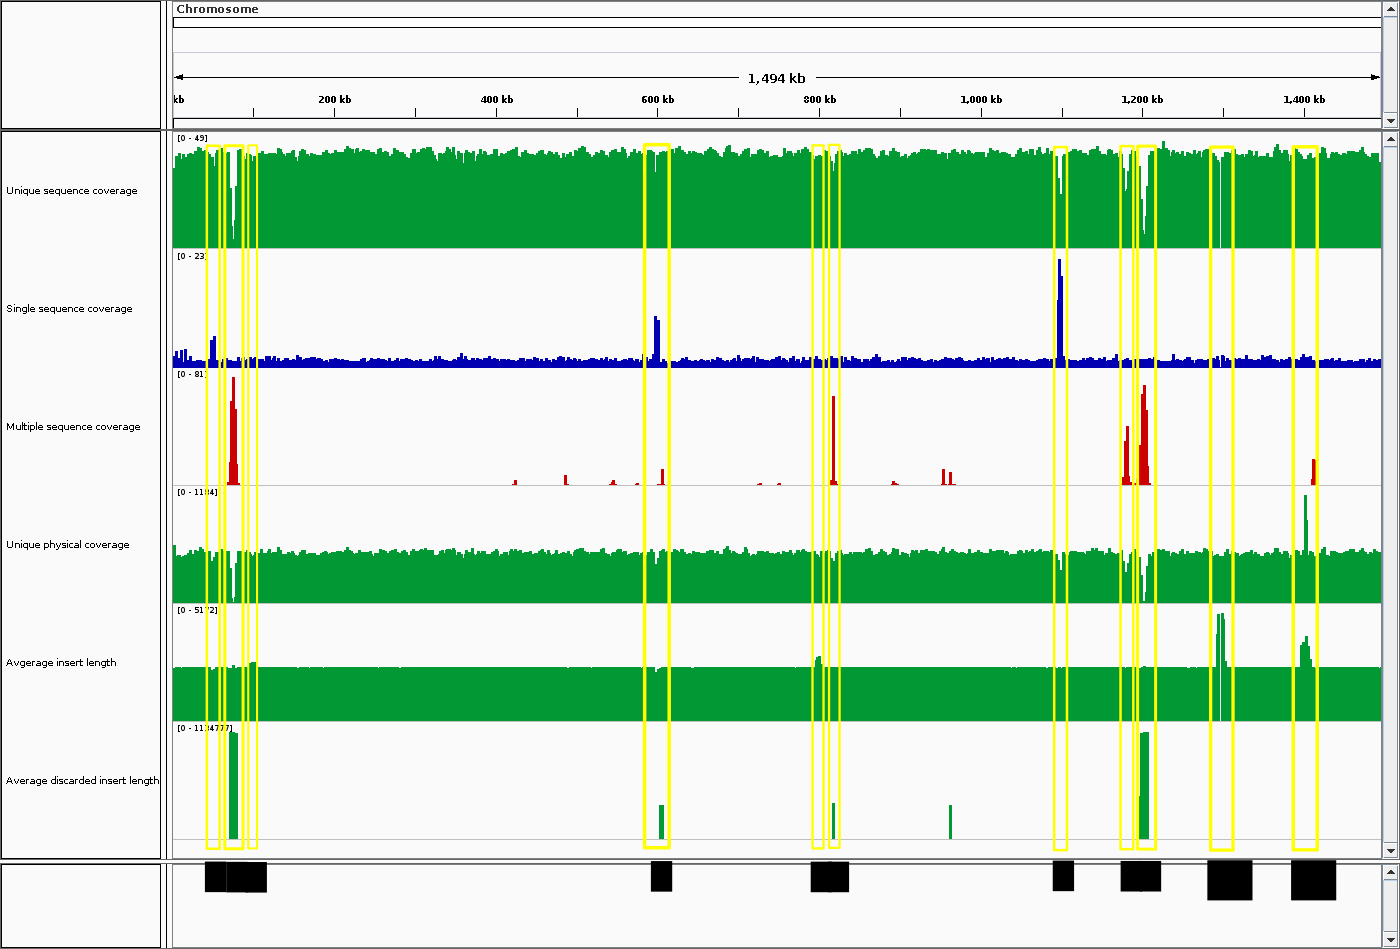
\includegraphics[width=\textwidth]{immagini/igv_global.png}
\caption{Vista globale delle tracce su IGV}
\label{fig:igv globale}
\end{figure}

La figura \ref{fig:igv globale} rappresenta le tracce appena descritte, i colori sono stati utilizzati per differenziare le tre tipologie di read a cui appartengono:
\begin{description}
\item[\textsc{Verde}]: identifica le tracce associate alle \emph{unique read};
\item[\textsc{Blu}]: identifica le tracce associate alle \emph{single read};
\item[\textsc{Rosso}]: identifica le tracce associate alle \emph{multiple read}.
\end{description}

Dai grafici si può notare come siano presenti diverse regioni interessanti all'interno delle tracce: sono quelle dove si vedono dei picchi in alcune di esse e avvallamenti nelle altre.

Le aree che a mio parere sono quelle più interessanti da valutare sono riquadrate con un rettangolo di colore giallo e per meglio identificarle sono numerate in ordine crescente.
Nel seguito verranno analizzate tali zone ed evidenziati i loro aspetti peculiari dando delle considerazioni sul possibile significato di variazione dei valori medi.
Le aree sono state raggruppate nel caso presentino aspetti comuni o pattern simili.

\subsection{Analisi regioni di interesse 1 e 4}
\begin{figure}[htbp]
\centering
\subfloat[][\emph{Regione 1}]
	{\includegraphics[width=.45\textwidth]{immagini/igv_regione1.png}} \quad
\subfloat[][\emph{Regione 4}]
	{\includegraphics[width=.45\textwidth]{immagini/igv_regione4.png}}
\caption{Regioni di interesse 1 e 4 su IGV}
\label{fig:regioni 1 e 4}
\end{figure}

In figura \ref{fig:regioni 1 e 4} si può notare come entrambe le regioni presentino due picchi nella \emph{sequence coverage} delle \emph{single read} mentre è presente una leggera diminuzione nella \emph{physical coverage} e in corrispondenza dei picchi la \emph{sequence coverage} delle \emph{unique read} presenta una leggera flessione: tale struttura potrebbe essere indicativa di brevi inserzioni dovute proprio alla presenza delle \emph{single read} e alla flessione della \emph{coverage}.

\subsection{Analisi regioni di interesse 2 e 9}
\begin{figure}[htbp]
\centering
\subfloat[][\emph{Regione 2}]
	{\includegraphics[width=.45\textwidth]{immagini/igv_regione2.png}} \quad
\subfloat[][\emph{Regione 9}]
	{\includegraphics[width=.45\textwidth]{immagini/igv_regione9.png}}
\caption{Regioni di interesse 2 e 9 su IGV}
\label{fig:regioni 2 e 9}
\end{figure}

Le immagini in figura \ref{fig:regioni 2 e 9} denotano la presenza di una notevole quantità di \emph{multiple read} che si sovrappone alla drastica diminuzione sia della \emph{physical} che della \emph{sequence coverage}.
Inoltre si può vedere come la lunghezza media degli inserti sia molto elevata.

Questi dati sono difficili da interpretare in quanto vi sarebbe la necessità di approfondire lo studio delle \emph{multiple read} per capire meglio le loro caratteristiche e individuare ulteriori \emph{mate pair}, se presenti.

\subsection{Analisi regioni di interesse 6 e 8}
\begin{figure}[htbp]
\centering
\subfloat[][\emph{Regione 6}]
	{\includegraphics[width=.45\textwidth]{immagini/igv_regione6.png}} \quad
\subfloat[][\emph{Regione 8}]
	{\includegraphics[width=.45\textwidth]{immagini/igv_regione8.png}}
\caption{Regioni di interesse 6 e 8 su IGV}
\label{fig:regioni 6 e 8}
\end{figure}

Le regioni in figura \ref{fig:regioni 6 e 8} presentano caratteristiche simili a quelle in \ref{fig:regioni 2 e 9} ma si distinguono in quanto presentano due brevi picchi di \emph{multiple read} distinti che comportano una diminuzione nella \emph{sequence coverage} delle \emph{unique read} e nella \emph{physical coverage}.

Anche in questo caso l'unico modo di capire meglio la situazione è quello di indagare più approfonditamente le \emph{multiple read}.

\subsection{Analisi regioni di interesse 3, 5 e 10}
\begin{figure}[htbp]
\centering
\subfloat[][\emph{Regione 3}]
	{\includegraphics[width=.45\textwidth]{immagini/igv_regione3.png}} \quad
\subfloat[][\emph{Regione 5}]
	{\includegraphics[width=.45\textwidth]{immagini/igv_regione5.png}} \\
\subfloat[][\emph{Regione 10}]
	{\includegraphics[width=.45\textwidth]{immagini/igv_regione10.png}}
\caption{Regioni di interesse 3, 5 e 10 su IGV}
\label{fig:regioni 3, 5 e 10}
\end{figure}

In figura \ref{fig:regioni 3, 5 e 10} troviamo dei casi molto simili: tutti e tre presentano zone in cui non sono presenti read e questo indica sicuramente delle cancellazioni nel genoma.
L'unica differenza degna di nota è l'ampiezza di tali cancellazioni, sulle regioni $3$ e $5$ si aggira tra le $500bp$ e le $1000bp$ mentre nella regione 10 è nettamente superiore misurando circa $5kbp$.

\subsection{Analisi regione di interesse 7}
\begin{figure}[htbp]
\centering
\includegraphics[width=.45\textwidth]{immagini/igv_regione7.png}
\caption{Regione di interesse 7 su IGV}
\label{fig:regione 7}
\end{figure}

La situazione rappresentata in figura \ref{fig:regione 7} è una chiara evidenza di una lunga inserzione in quanto si vede la \emph{physical coverage} creare il tipico aspetto a \emph{V} e la \emph{sequence coverage} delle \emph{unique read} scendere molto e quella delle \emph{single read} essere molto alta.

\subsection{Analisi regione di interesse 11}
\begin{figure}[htbp]
\centering
\includegraphics[width=.45\textwidth]{immagini/igv_regione11.png}
\caption{Regione di interesse 11 su IGV}
\label{fig:regioni 11}
\end{figure}

L'immagine in figura \ref{fig:regioni 11} presenta invece un aspetto per me insolito in quanto presenta una forma a \emph{V} rovesciata in concomitanza di aumenti sensibili e simmetrici della lunghezza media degli inserti.
%\clearpage
\section{Conclusioni}
L'analisi effettuata mediante questo progetto non può certo dirsi esaustiva in quanto sarebbe possibile approfondire alcuni aspetti che non ho trattato: d'altronde il tempo a disposizione non era molto e lo studio iniziale ha richiesto notevole impegno prima di iniziare a produrre i primi risultati.

Nonostante tutto devo dire di aver appreso molto meglio alcuni concetti che durante lo studio delle lezioni mi erano meno chiari o che credevo di aver capito bene e si sono rivelati essere approssimativi.

Sono quindi molto soddisfatto del lavoro che ho svolto anche se non ho la certezza di non aver commesso alcuni errori nel calcolare i risultati o nell'interpretarli nel modo corretto.

\end{document}